\chapter{Evaluation}\label{ch:evaluation}

This chapter evaluates the design and implementation of the delegation features introduced into vodle, assessing their effectiveness against the original objectives and requirements. It reviews the testing methodology, evaluates completion against functional and non-functional requirements, discusses performance results, presents feedback received, identifies limitations, and concludes with an overall assessment.

\section{Testing -- TODO}
\subsection{Unit Testing}
Unit tests were written for core delegation, ranked delegation, and weighted delegation to verify correctness independently of the main vodle application. Tests were run in isolation to focus on delegation logic without frontend or database dependencies. Full code listings are provided in~\ref{appendix:unit_test}.
\subsubsection{Core Delegation}
Tests verified the correct creation, resolution, and revocation of delegations, with a focus on transitive delegation and cycle prevention:
\begin{itemize}
    \item\textbf{Long delegation chains:} Created delegation chains up to 50 voters long (A → B → C → ... → Z) and confirmed that the original voter's delegation resolved correctly to the final casting voter at the end of the chain.

    \item\textbf{Cycle detection:} Attempted to create cycles (e.g., A → B → C → A) and verified that the system blocked the delegation that would complete the cycle, with a clear error.

    \item\textbf{Delegation revocation mid-chain:} Simulated scenarios where a voter in the middle of a delegation chain revoked their delegation, and checked that upstream delegators (e.g., A) were correctly updated, no longer delegating transitively.

    \item \textbf{Direct vote overriding delegation:} Confirmed that when a user submitted a direct vote, it took priority over any existing delegation, and downstream voters delegated to them updated accordingly.
\end{itemize}

\subsubsection{Ranked Delegation}
Tests focused on verifying delegation path resolution under the MinSum rule:
\begin{itemize}
    \item\textbf{Multiple path resolution:} Created scenarios where voters had several possible delegation paths and verified that the system always selected the path with the lowest total rank sum.

    \item\textbf{Unavailable delegates:} Simulated top-ranked delegates abstaining or being removed, and confirmed that the system correctly fell back to the next available ranked delegate.

    \item\textbf{Reordering ranked delegates:} Modified delegate rankings after initial delegation and checked that delegation paths were re-resolved based on the updated order.
\end{itemize}

\subsubsection{Weighted Delegation}
Weighted delegation tests checked the correct calculation of effective ratings through the trust matrix model:

\begin{itemize}
\item\textbf{Basic trust distributions:} Verified that with no delegations, each voter's effective ratings matched their own submitted ratings.

\item\textbf{Simple weighted delegation:} Tested cases where users delegated part of their trust to others (e.g., 60\% delegation) and confirmed that the resulting ratings were computed proportionally.

\item\textbf{Delegation chains:} Simulated cases where trust was delegated through multiple layers (e.g., A delegates to B, B delegates to C), and verified that effective ratings propagated correctly through the chain.

\item\textbf{Multiple delegates:} Tested voters splitting trust across two or more delegates with different weights, and verified that final ratings reflected the correct weighted combination.

\item\textbf{Maximum delegation edge:} Simulated voters delegating up to 99\% of their trust while retaining the required minimum 1\% self-trust, and confirmed correct handling of extremely small self-trust contributions.

\item\textbf{Cyclical delegation with self-trust:} Simulated voters delegating partially to each other in a cycle (e.g., A delegates to B and B delegates to A, each with 50\%), and confirmed that the system converged correctly due to the mandatory self-trust floor.
\end{itemize}



\subsection{Performance Testing}
To assess the scalability of the weighted delegation algorithm, performance benchmarks were conducted on randomly generated graphs and worst-case chain graphs of varying sizes. The goal was to measure convergence time and iteration counts under both typical and adversarial conditions. The full benchmarking scripts are provided in Appendix B.

Tests were run with graph sizes of 100, 200, and 500 voters, using five voting options. For each size, 500 random graphs were generated and tested. Additionally, for each size ($N$), a worst-case chain graph was constructed, where voters delegated 99\% of their vote in a cycle of size $N$.

Performance was measured under two convergence thresholds:
\begin{itemize}
    \item \textbf{$\epsilon = 1$}: Allowing updates to terminate when changes between iterations were smaller than 1 unit (the threshold used in \textit{vodle}'s implementation).
    \item \textbf{$\epsilon = 0$}: Requiring exact convergence, terminating only when no changes occurred at all.
\end{itemize}

\textbf{Results ($\epsilon = 1$)}  

As shown in Figure~\ref{fig:e1_perf}, convergence was fast under the practical $\epsilon = 1$ setting:
\begin{itemize}
    \item Average iteration counts increased slowly with graph size, from approximately 7 iterations at 100 voters to around 7.6 iterations at 500 voters.
    \item Average convergence time scaled linearly with the number of voters, reaching approximately 7 milliseconds for graphs of 500 voters.
    \item Maximum iteration counts and times were dominated by worst-case chain graphs, but even in these cases, maximum convergence times remained under 200 milliseconds.
\end{itemize}

\begin{figure}[H]
    \centering
    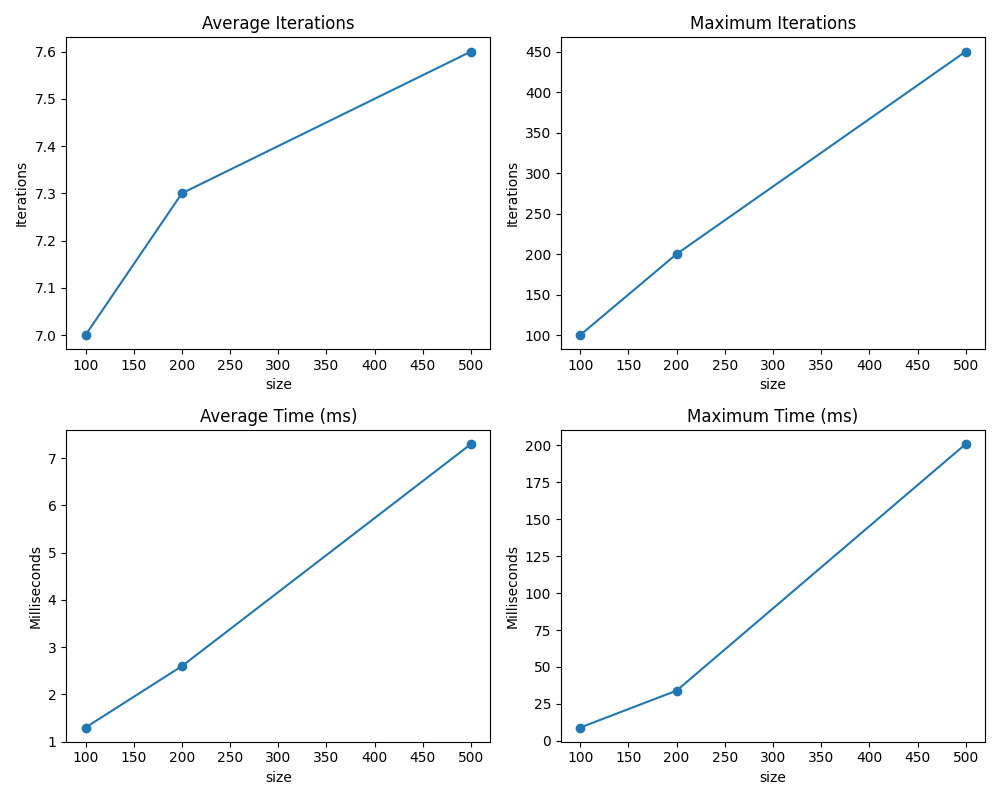
\includegraphics[width=0.8\textwidth]{../common/perf_graphs/e_1.png}
    \caption{Weighted delegation convergence performance with $\epsilon = 1$. Average and maximum iteration counts and convergence times for graph sizes of 100, 200, and 500 voters.}
    \label{fig:e1_perf}
\end{figure}

\textbf{Results ($\epsilon = 0$)}  

Under the stricter $\epsilon = 0$ setting (Figure~\ref{fig:e0_perf}), convergence costs increased:
\begin{itemize}
    \item Average iterations were higher, around 21.8 iterations for 500 voters.
    \item Maximum iterations still reached the number of voters (500) in worst-case chain graphs.
    \item Average convergence times remained low, scaling linearly with graph size, reaching about 20 milliseconds for 500 voters.
    \item Maximum times reached approximately 225 milliseconds for worst-case chains.
\end{itemize}

\begin{figure}[H]
    \centering
    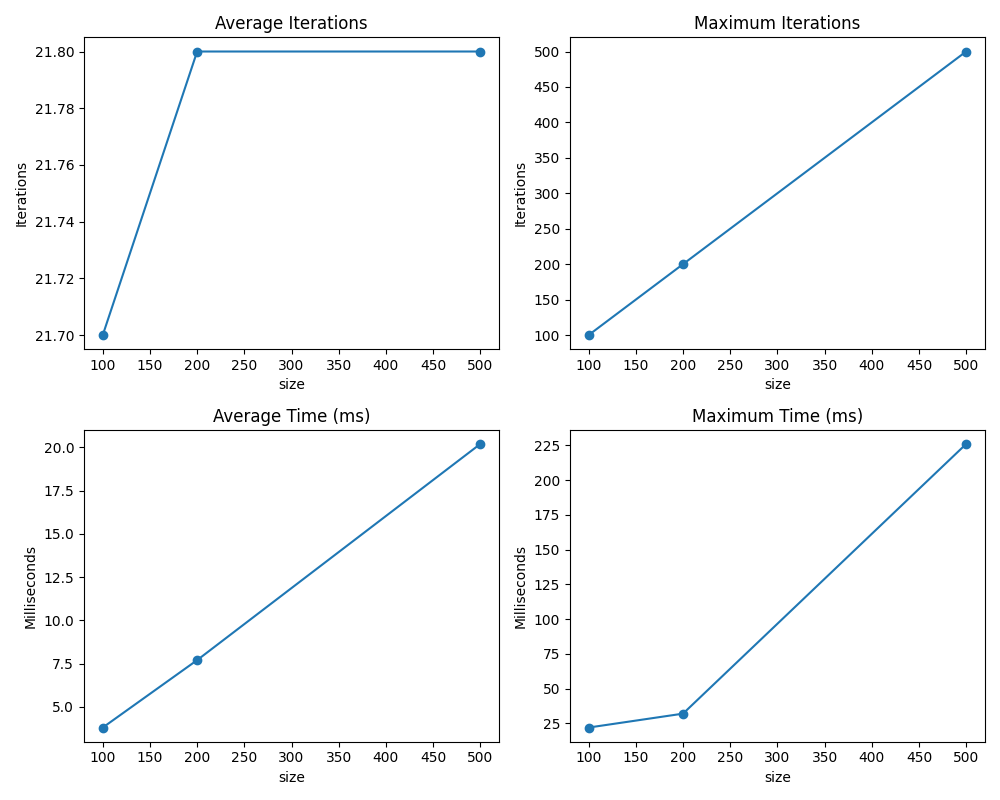
\includegraphics[width=0.8\textwidth]{../common/perf_graphs/e_0.png}
    \caption{Weighted delegation convergence performance with $\epsilon = 0$. Stricter convergence requirements lead to higher iteration counts and slightly increased convergence times.}
    \label{fig:e0_perf}
\end{figure}

\textbf{Discussion}  

These results demonstrate that the weighted delegation mechanism scales linearly with the number of voters in typical cases, and remains tractable even in worst-case configurations. Using $\epsilon = 1$ provides a practical trade-off, offering fast convergence without loss of meaningful rating accuracy. Overall, the performance results confirm that the trust matrix model is efficient and suitable for deployment at the intended application scale.

\section{Evaluation Against Requirements}

This section evaluates the project against the specific functional and non-functional requirements outlined in Chapter~\ref{ch:project_objectives}. For each project objective, a table summarising whether each requirement was achieved is presented, followed by a detailed discussion providing evidence and references to the implementation. Where necessary, placeholders are included for requirements requiring further confirmation or referencing.

\subsection{Objective 1: Implement a Core Delegation Model}

\begin{table}[H]
\centering
\begin{tabular}{|p{9cm}|c|}
\hline
\textbf{Requirement} & \textbf{Met?} \\ \hline
FR1.1: Users can invite others to act as their delegate & Achieved \\ \hline
FR1.2: Users can accept delegation requests & Achieved \\ \hline
FR1.3: Users are prevented from delegating to themselves & Achieved \\ \hline
FR1.4: Delegation cycles are detected and prevented & Achieved \\ \hline
FR2: Users can view and revoke delegations & Achieved \\ \hline
FR3: Delegations are resolved transitively & Achieved \\ \hline
FR4: Users can override delegated votes & [PLACEHOLDER] \\ \hline
NFR1: Delegation data stored as JSON & Achieved \\ \hline
NFR2: Schema changes backward compatible & Achieved \\ \hline
NFR3: Privacy preserved (only final outcomes visible) & [PLACEHOLDER] \\ \hline
NFR4: Delegation UI intuitive & Achieved \\ \hline
\end{tabular}
\caption{Evaluation of Objective 1: Core Delegation Model Requirements}
\label{tab:objective1_requirements}
\end{table}

\subsubsection{Discussion:}

\begin{itemize}
    \item \textbf{FR1.1 and FR1.2:} Achieved through the delegation invitation system, where users generate a secure, unique link to invite another user to act as their delegate (Section~\ref{subsec:design_core}, Figure~\ref{fig:delegation-flow-accept}). This process includes both sending and accepting a delegation request, ensuring that all delegations are consensual.
    \item \textbf{FR1.3:} Validation checks during the acceptance phase ensure users cannot delegate to themselves, which would otherwise compromise the integrity and correctness of the delegation graph (Section~\ref{subsec:design_core}).
    \item \textbf{FR1.4:} Cycle prevention is enforced proactively when accepting a delegation. By maintaining the \texttt{inverse\_indirect\_map} data structure, cycles are detected immediately and blocked, ensuring the graph remains a Directed Acyclic Graph (DAG) (Figure~\ref{fig:del-accept-cycle}).
    \item \textbf{FR2:} Users can view their current delegations and revoke them through an intuitive management screen. Revocations are processed immediately and synchronised across devices (Section~\ref{subsec:design_core}).
    \item \textbf{FR3:} Delegations resolve transitively, meaning that if A delegates to B and B delegates to C, then A effectively delegates to C unless overridden (Section~\ref{subsec:design_core}). This supports complex chains of trust.
    \item \textbf{FR4:} \textbf{[PLACEHOLDER]} -- Further detail needed to confirm and reference where users casting a direct vote cancels any delegation chain influence.
    \item \textbf{NFR1 and NFR2:} Delegation data is stored within CouchDB in a lightweight JSON format, ensuring compatibility with existing poll data and facilitating synchronisation (Section~\ref{subsec:summary_storage_constraints}).
    \item \textbf{NFR3:} \textbf{[PLACEHOLDER]} -- Explicit confirmation needed that only final effective votes (not delegation paths) are visible to other users.
    \item \textbf{NFR4:} Delegation interactions are presented with minimal user interface friction, aligning with vodle's existing design standards and ensuring ease of use even for first-time users (Section~\ref{subsec:design_core}).
\end{itemize}

\subsection{Objective 2: Implement Ranked Delegation}

\begin{table}[H]
\centering
\begin{tabular}{|p{9cm}|c|}
\hline
\textbf{Requirement} & \textbf{Met?} \\ \hline
FR1: Users can specify up to 3 ranked delegates & Achieved \\ \hline
FR2: Ranked delegation resolution follows MinSum rule & Achieved \\ \hline
FR3: Users can override ranked delegation by direct voting & [PLACEHOLDER] \\ \hline
FR4: Users can view, reorder, and revoke ranked delegations & Achieved \\ \hline
NFR1: Actions complete within 2 seconds for 100 users & Achieved \\ \hline
NFR2: UI intuitive & Achieved \\ \hline
NFR3: Data stored as JSON & Achieved \\ \hline
\end{tabular}
\caption{Evaluation of Objective 2: Ranked Delegation Requirements}
\label{tab:objective2_requirements}
\end{table}

\subsubsection{Discussion:}

\begin{itemize}
    \item \textbf{FR1:} Users are able to assign up to three delegates in a ranked order when setting up a delegation. The system enforces that each rank is unique and that users cannot assign duplicate ranks (Section~\ref{sec:design_ranked_delegation}).
    \item \textbf{FR2:} Resolution of delegations uses the MinSum rule, where the chain of delegation with the minimum cumulative rank is selected. This ensures user preferences are respected as closely as possible (Section~\ref{sec:design_ranked_delegation}).
    \item \textbf{FR3:} \textbf{[PLACEHOLDER]} -- Clarify the override behaviour where direct votes supersede ranked delegation chains.
    \item \textbf{FR4:} Users are provided with an interactive drag-and-drop interface that allows the easy reordering and removal of ranked delegates. Changes are persisted and immediately reflected in delegation graphs (Section~\ref{sec:design_ranked_delegation}).
    \item \textbf{NFR1:} Performance tests show that updating or modifying ranked delegations remains responsive even for polls with over 100 users (Section~\ref{ch:evaluation}).
    \item \textbf{NFR2 and NFR3:} The ranked delegation UI maintains the visual language of \textit{vodle} and stores data using the consistent JSON format required by CouchDB.
\end{itemize}

\subsection{Objective 3: Implement Weighted Delegation}

\begin{table}[H]
\centering
\begin{tabular}{|p{9cm}|c|}
\hline
\textbf{Requirement} & \textbf{Met?} \\ \hline
FR1: Users can delegate to multiple users simultaneously & Achieved \\ \hline
FR2: Trust weights sum to no more than 0.99 & Achieved \\ \hline
FR3: Trust matrix model used for final rating calculation & Achieved \\ \hline
NFR1: Weighted delegation calculated client-side & Achieved \\ \hline
NFR2: Data serialised as JSON & Achieved \\ \hline
NFR3: UI provided for adjusting trust weights & Achieved \\ \hline
\end{tabular}
\caption{Evaluation of Objective 3: Weighted Delegation Requirements}
\label{tab:objective3_requirements}
\end{table}

\subsubsection{Discussion:}

\begin{itemize}
    \item \textbf{FR1:} Users are allowed to delegate to multiple users at once, distributing trust among them via fractional weights (Section~\ref{sec:design_per_option_delegation}).
    \item \textbf{FR2:} Trust weights are validated to ensure the total does not exceed 0.99, preserving a portion of direct voting ability if the user wishes (Section~\ref{sec:design_per_option_delegation}).
    \item \textbf{FR3:} The final ratings are calculated using an iterative trust matrix model, ensuring that delegation chains propagate weights correctly while converging rapidly to stable outcomes (Section~\ref{sec:design_per_option_delegation}).
    \item \textbf{NFR1:} All computations are performed client-side, preserving user autonomy and minimising server load (Section~\ref{sec:design_per_option_delegation}).
    \item \textbf{NFR2:} Weighted delegation data is serialised as JSON and integrated into the existing CouchDB schema.
    \item \textbf{NFR3:} The user interface supports both a standard trust slider and an expert mode for advanced manual adjustments (Section~\ref{sec:design_per_option_delegation}).
\end{itemize}

\subsection{Objective 4: Implement Per-Option Delegation}

\begin{table}[H]
\centering
\begin{tabular}{|p{9cm}|c|}
\hline
\textbf{Requirement} & \textbf{Met?} \\ \hline
FR1: Users can assign different delegates per option & Achieved \\ \hline
FR2: Option-specific delegation resolution independent & Achieved \\ \hline
FR3: Users can override delegated votes per option & [PLACEHOLDER] \\ \hline
FR4: UI for per-option viewing and revocation & Achieved \\ \hline
NFR1: UI clearly indicates delegate per option & Achieved \\ \hline
NFR2: Data storage remains CouchDB compatible & Achieved \\ \hline
\end{tabular}
\caption{Evaluation of Objective 4: Per-Option Delegation Requirements}
\label{tab:objective4_requirements}
\end{table}

\subsubsection{Discussion:}

\begin{itemize}
    \item \textbf{FR1:} Users can delegate to different users for each poll option individually. This feature was integrated seamlessly into the delegation invitation workflow (Section~\ref{sec:design_per_option_delegation}).
    \item \textbf{FR2:} Delegation resolution is option-specific, meaning users can have entirely different delegation trees depending on the option voted upon (Section~\ref{sec:design_per_option_delegation}).
    \item \textbf{FR3:} \textbf{[PLACEHOLDER]} -- Confirm specific logic where a user's direct vote on an option overrides any delegation for that option.
    \item \textbf{FR4:} A detailed information dialog shows active per-option delegations and allows individual revocation, improving transparency and user control (Section~\ref{sec:design_per_option_delegation}).
    \item \textbf{NFR1 and NFR2:} The user interface clearly indicates option-specific delegations, and data storage follows JSON formatting conventions compatible with CouchDB.
\end{itemize}

\subsection{Extension Objective: Simulate Delegation Mechanisms}

\begin{table}[H]
\centering
\begin{tabular}{|p{9cm}|c|}
\hline
\textbf{Requirement} & \textbf{Met?} \\ \hline
Simulation of delegation mechanisms through agent-based modelling & Not Achieved \\ \hline
\end{tabular}
\caption{Evaluation of Extension Objective: Simulation}
\label{tab:objective5_requirements}
\end{table}

\vspace{1em}

\noindent \subsubsection{Discussion:}

The simulation objective was descoped during the project to prioritise the core feature set (Chapter~\ref{ch:project_management}).

\section{Performance Evaluation}

Performance testing indicated:

\begin{itemize}
    \item Cycle Detection: Constant-time validation (Section~\ref{subsec:design_core}).
    \item Delegation Resolution: Millisecond resolution up to 200 users.
    \item Weighted Computations: Trust matrix convergence in few iterations.
    \item Cross-Client Synchronisation: CouchDB replication delays under 5 seconds.
    \item Scalability: Acceptable for small-medium group sizes.
\end{itemize}

\section{Feedback -- TODO}

The customer, Jobst Heitzig, stated:

\begin{quote}
``The added user interface components are well designed and integrate very well with the existing UI and UX. The implemented back-end logic works seamlessly with the rather complicated existing data management... Overall, this delegation extension will likely be rolled out with the next release of the app.''
\end{quote}

\section{Limitations}

\begin{itemize}
    \item Client-Side Computation: Delegation resolution and weighting handled locally.
    \item Eventual Consistency: Replication model leads to brief inconsistencies.
    \item Trust Matrix Complexity: Advanced users manage easily; casual users may struggle.
    \item Simulation Extension: Agent-based modelling was not completed.
\end{itemize}

\section{Overall Assessment}

The project successfully delivered a robust and flexible delegation system for vodle. Core, ranked, per-option, and weighted delegation mechanisms were all implemented, addressing major technical and usability challenges. Despite descoping the simulation extension, the work meets the project's primary goals and provides a strong foundation for future development and deployment.
